\documentclass{article}

% Packages required to support encoding
\usepackage{ucs}
\usepackage[utf8x]{inputenc}
\usepackage{graphicx} 
% Packages required by code


% Packages always used
\usepackage{hyperref}
\usepackage{xspace}
\usepackage[usenames,dvipsnames]{color}
\hypersetup{colorlinks=true,urlcolor=blue}


\usepackage{geometry}
\geometry{letterpaper,textwidth=350pt,textheight=680pt,tmargin=60pt,
            left=72pt,footskip=24pt,headsep=18pt,headheight=14pt}
\usepackage{amsmath}
\usepackage{amssymb}
\usepackage{textcase}
\usepackage{soul}

\newcommand{\mat}[1]{\boldsymbol{#1}}\renewcommand{\vec}[1]{\boldsymbol{\mathrm{#1}}}
\newcommand{\vecalt}[1]{\boldsymbol{#1}}

\newcommand{\conj}[1]{\overline{#1}}

\newcommand{\normof}[1]{\|#1\|}
\newcommand{\onormof}[2]{\|#1\|_{#2}}

\newcommand{\itr}[2]{#1^{(#2)}}
\newcommand{\itn}[1]{^{(#1)}}

\newcommand{\eps}{\varepsilon}
\newcommand{\kron}{\otimes}

\DeclareMathOperator{\diag}{diag}
\DeclareMathOperator{\trace}{trace}
\DeclareMathOperator{\tvec}{vec}

\newcommand{\prob}{\mathbb{P}}
\newcommand{\probof}[1]{\prob\left\{ #1 \right\}}

\newcommand{\pmat}[1]{\begin{pmatrix} #1 \end{pmatrix}}
\newcommand{\bmat}[1]{\begin{bmatrix} #1 \end{bmatrix}}
\newcommand{\spmat}[1]{\left(\begin{smallmatrix} #1 \end{smallmatrix}\right)}
\newcommand{\sbmat}[1]{\left[\begin{smallmatrix} #1 \end{smallmatrix}\right]}

\newcommand{\RR}{\mathbb{R}}
\newcommand{\CC}{\mathbb{C}}

\providecommand{\eye}{\mat{I}}
\providecommand{\mA}{\ensuremath{\mat{A}}}
\providecommand{\mB}{\ensuremath{\mat{B}}}
\providecommand{\mC}{\ensuremath{\mat{C}}}
\providecommand{\mD}{\ensuremath{\mat{D}}}
\providecommand{\mE}{\ensuremath{\mat{E}}}
\providecommand{\mF}{\ensuremath{\mat{F}}}
\providecommand{\mG}{\ensuremath{\mat{G}}}
\providecommand{\mH}{\ensuremath{\mat{H}}}
\providecommand{\mI}{\ensuremath{\mat{I}}}
\providecommand{\mJ}{\ensuremath{\mat{J}}}
\providecommand{\mK}{\ensuremath{\mat{K}}}
\providecommand{\mL}{\ensuremath{\mat{L}}}
\providecommand{\mM}{\ensuremath{\mat{M}}}
\providecommand{\mN}{\ensuremath{\mat{N}}}
\providecommand{\mO}{\ensuremath{\mat{O}}}
\providecommand{\mP}{\ensuremath{\mat{P}}}
\providecommand{\mQ}{\ensuremath{\mat{Q}}}
\providecommand{\mR}{\ensuremath{\mat{R}}}
\providecommand{\mS}{\ensuremath{\mat{S}}}
\providecommand{\mT}{\ensuremath{\mat{T}}}
\providecommand{\mU}{\ensuremath{\mat{U}}}
\providecommand{\mV}{\ensuremath{\mat{V}}}
\providecommand{\mW}{\ensuremath{\mat{W}}}
\providecommand{\mX}{\ensuremath{\mat{X}}}
\providecommand{\mY}{\ensuremath{\mat{Y}}}
\providecommand{\mZ}{\ensuremath{\mat{Z}}}
\providecommand{\mLambda}{\ensuremath{\mat{\Lambda}}}
\providecommand{\mPbar}{\bar{\mP}}

\providecommand{\ones}{\vec{e}}
\providecommand{\va}{\ensuremath{\vec{a}}}
\providecommand{\vb}{\ensuremath{\vec{b}}}
\providecommand{\vc}{\ensuremath{\vec{c}}}
\providecommand{\vd}{\ensuremath{\vec{d}}}
\providecommand{\ve}{\ensuremath{\vec{e}}}
\providecommand{\vf}{\ensuremath{\vec{f}}}
\providecommand{\vg}{\ensuremath{\vec{g}}}
\providecommand{\vh}{\ensuremath{\vec{h}}}
\providecommand{\vi}{\ensuremath{\vec{i}}}
\providecommand{\vj}{\ensuremath{\vec{j}}}
\providecommand{\vk}{\ensuremath{\vec{k}}}
\providecommand{\vl}{\ensuremath{\vec{l}}}
\providecommand{\vm}{\ensuremath{\vec{l}}}
\providecommand{\vn}{\ensuremath{\vec{n}}}
\providecommand{\vo}{\ensuremath{\vec{o}}}
\providecommand{\vp}{\ensuremath{\vec{p}}}
\providecommand{\vq}{\ensuremath{\vec{q}}}
\providecommand{\vr}{\ensuremath{\vec{r}}}
\providecommand{\vs}{\ensuremath{\vec{s}}}
\providecommand{\vt}{\ensuremath{\vec{t}}}
\providecommand{\vu}{\ensuremath{\vec{u}}}
\providecommand{\vv}{\ensuremath{\vec{v}}}
\providecommand{\vw}{\ensuremath{\vec{w}}}
\providecommand{\vx}{\ensuremath{\vec{x}}}
\providecommand{\vy}{\ensuremath{\vec{y}}}
\providecommand{\vz}{\ensuremath{\vec{z}}}
\providecommand{\vpi}{\ensuremath{\vecalt{\pi}}}

\sodef\allcapsspacing{\upshape}{0.15em}{0.65em}{0.6em}%

\makeatletter
\def\maketitle{%
\par
\hrule height 0.75pt\vspace{1ex}
\par\noindent
\begin{minipage}{0.5\textwidth}
\scshape
purdue university $\cdot$ CS 580 \\
Introduction to the Analysis of Algorithms
\end{minipage}
\begin{minipage}{0.5\textwidth}
\raggedleft
\MakeTextUppercase{\allcapsspacing{\@title}}\\[0.2ex]
\textit{\@author}\\[0.2ex]
\textit{\@date}
\end{minipage}
\par\vspace{1ex}
\hrule height 1pt
\vspace{2ex}
\par
}
\makeatother

\author{Jun Cheng}
\title{Lecture Notes}
% auto generate a title
\AtBeginDocument{\maketitle}


\title{Homework}



\begin{document} 



\hypertarget{problem_0_homework_checklist_2}{}\subsection*{{Problem 0: Homework checklist}}\label{problem_0_homework_checklist_2}

\checkmark	I didn't talk with any one about this homework. \newline
\checkmark 	Source-code are included at the end of this document. 


\hypertarget{problem_1_operations_3}{}\subsection*{{Problem 1: Operations}}\label{problem_1_operations_3}



1. $\bmat{ 1 & 1 & 2 \\ 3 & 5 & 8 \\ 13 & 21 & 34 } \bmat{ 1 & -2 & 3 \\ -4 & 5 & -6 \\ 7 & -8 & 9} =\bmat{11 & -13 & 15 \\ 39 & -45 & 51 \\ 167 & -193 & 219}$ \newline

2. $\vx =$ {\colorbox[rgb]{1.00,0.93,1.00}{\tt ones\char40\char49\char48\char48\char48\char44\char49\char41}} $\vy =$ {\colorbox[rgb]{1.00,0.93,1.00}{\tt \char91\char49\char58\char49\char48\char48\char48\char93\char39}} $\vx^T \vy =$ 500500.0 \newline


\hypertarget{problem_4_image_downsampling_6}{}\subsection*{{Problem 4: Image downsampling}}\label{problem_4_image_downsampling_6}

1.%$\vy \in \RR^{4}$   
$\vy = \mA\vx $
so A must be a $4\times 16$ matrix.  $ y_i= \sum_{j=1}^{16}A_{ij}x_j  $ \\
$ y_1 = (x_1 + x_2 + x_5 + x_6)/4 $ \newline
$ y_2 = (x_3 + x_4 + x_7 + x_8)/4   $ \newline
$ y_3 = (x_9 + x_{10} + x_{13} + x_{14})/4 $ \newline
$ y_4 = (x_{11} + x_{12} + x_{15} + x_{16})/4.$ \newline

Then\\ $ \mA_{11}= \mA_{12}= \mA_{15}= \mA_{16} = 0.25 $\\
$ \mA_{23}= \mA_{24}= \mA_{27}= \mA_{28} = 0.25 $\\
$ \mA_{39}= \mA_{3,10}= \mA_{3,13}= \mA_{3,14} = 0.25 $\\
$ \mA_{4,11}= \mA_{4,12}= \mA_{4,15}= \mA_{4,16} = 0.25 $\\

\begin{equation*}\mA=
\left[
\begin{array}{cccccccccccccccc}
0.25 & 0.25 & 0 & 0 & 0.25 & 0.25 & 0 & 0 & 0 & 0 & 0 & 0 & 0 & 0 & 0 & 0  \\
0 & 0 & 0.25 & 0.25 & 0 & 0 & 0.25 & 0.25 & 0 & 0 & 0 & 0 & 0 & 0 & 0 & 0  \\
0 & 0 & 0 & 0 & 0 & 0 & 0 & 0 & 0.25 & 0.25 & 0 & 0 & 0.25 & 0.25 & 0 & 0 \\
0 & 0 & 0 & 0 & 0 & 0 & 0 & 0 & 0 & 0 & 0.25 & 0.25 & 0 & 0 & 0.25 & 0.25 \\
\end{array}
\right]
\end{equation*}
2. The sum of diagonal elements of $X$ is 24.2686  \\

3.  Color image:  
Grey image: 
\begin{figure} [h]
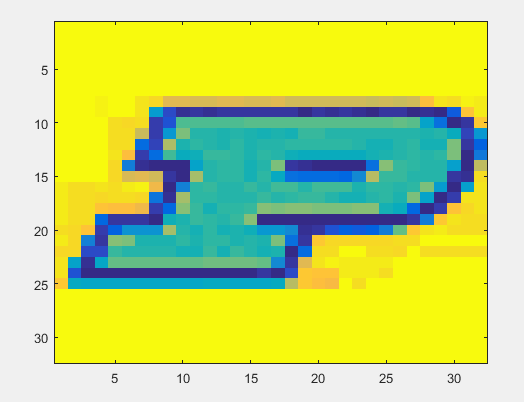
\includegraphics[width=8cm]{color}
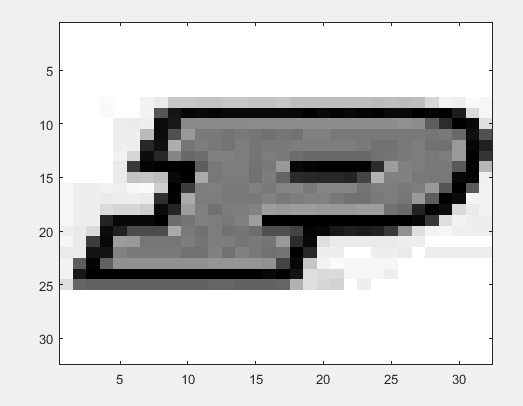
\includegraphics[width=8cm]{gray}
\end{figure}

4.  Resahpe command will reshape the input array into a $m\times n$ matrix, and return the new matrix. 





\end{document} 



